\subsection{Results}

\subsubsection{GemNet}

We evaluated the GemNet model on the S2EF task with the 200k dataset and
the IS2RE task with the 100k dataset. For both tasks, we trained for one epoch
using a batch size of 16 (since data parallelism was activated in all of the 
runs, this implies that each of the 8 GPUs received 2 molecules per forward pass). 

We evaluated the GPU memory consumed by CUDA tensors and runtimes for GemNet training with 8 different 
configurations of DeepSpeed:
The so-called DeepSpeed ZeRO stage 0 served as baseline for evaluations, in which 
all DeepSpeed optimizations are deactivated---i.e. stage 0 corresponds to basic 
data-parallel training. As a second configuration, we trained GemNet 
in half precision without any ZeRO optimizations in order to make sure that
potential memory savings by ZeRO are actually caused by the model state partitioning and
not merely by reducing the model parameters' precision.

Apart from this, we evaluated two configurations of each stage of ZeRO-DP to benchmark 
them against the two baselines. More precisely, for stage 1, we did one run with and 
without overlapping communication each, while overlapping communication
was activated throughout stage 2 and stage 3. In order to investigate potential 
memory savings by CPU offloading, we conducted standard stage 2 and stage 3 runs as well
as runs in which the respective maximal CPU offloading capacity was exploited.
The exact configurations and results can be seen in Figure~\ref{fig:gemnet-s2ef}
and Figure~\ref{fig:gemnet-is2re}, where \enquote{OC} stands for overlapping communication,
\enquote{OO} for optimizer offloading and \enquote{PO} for parameter offloading.

When comparing stage 0 with half precision to standard stage 1, a significant decrease
both in allocated GPU memory and reserved GPU memory can be observed for both S2EF and IS2RE
(S2EF: -67\% allocated, -23\% reserved; IS2RE: -78\% allocated, -12\% reserved).
This drop in memory consumption has to be caused by optimizer state partitioning among
the GPUs since this is the only difference between the configurations. 
Both for the S2EF task and the IS2RE task, forward and backward pass---excluding communication
---are marginally faster with stage 1 activated. 

However, especially for the S2EF task, it is also clearly visible that communication overhead 
between the GPUs rises for stage 1: The part of the total epoch runtime which
neither belongs to one of the tracked stages (calles \enquote{rest} in 
Figure~\ref{fig:gemnet-s2ef} and Figure~\ref{fig:gemnet-is2re}) and thus mainly 
encompass communication, increases by 219\% (S2EF) and 58\% (IS2RE).

Additionally, CPU offloading saves memory---most notable is a 58\% decrease of allocated GPU 
memory with IS2RE when optimizer offloading is activated in stage 2. Nevertheless,
in all of the observed cases this came at the cost of increased runtime.

Stage 3 seems to be ineffective for GemNet as neither memory footprints nor 
runtime are improved. Likewise, communication overlapping (which we had hoped would
reduce runtime) did not have the desired effect as can be seen from the comparison 
between the two stage 1 runtimes.

\begin{figure}[H]
    \centering

    \begin{subfigure}[t]{0.48\textwidth}
        \centering
        \includegraphics[width=\textwidth]{evaluation/gemnet/s2ef/cuda_memory/memory_comparison.pdf}
    \end{subfigure}%
    ~
    \begin{subfigure}[t]{0.48\textwidth}
        \centering
        \includegraphics[width=\textwidth]{evaluation/gemnet/s2ef/runtimes/runtimes_comparison.pdf}
    \end{subfigure}

    \resizebox{0.95\textwidth}{!}{%
    \begin{tabular}{ll|l|l|l|l|l|l|l|l|}
    \cline{3-10}
    & & \scriptsize \textbf{S0}    & \scriptsize \textbf{S0}+fp16 & \scriptsize \textbf{S1}             & \scriptsize \textbf{S1}+OC          & \scriptsize \textbf{S2}+OC & \begin{tabular}{@{}c@{}}\scriptsize\textbf{S2}+OO \vspace*{-0.5em} \\ \scriptsize+OC\end{tabular}      & \scriptsize \textbf{S3}+OC & \scriptsize \begin{tabular}{@{}c@{}}\scriptsize\textbf{S3}+PO \\ \scriptsize+OO+OC\end{tabular} \\ \hline \hline
    \multicolumn{1}{|l|}{\multirow{2}{*}{memory}}   & allocated   & 7.11     & 7.1               & 2.36           & 2.36              & 2.36     & \textbf{1.78} & 3.51     & 2.78              \\ \cline{2-10} 
    \multicolumn{1}{|l|}{}                          & reserved    & 37.71    & 24.98             & \textbf{18.99} & \textbf{18.99}    & 20.3     & 19.77         & 21.99    & 21.32             \\ \hline \hline
    \multicolumn{1}{|l|}{\multirow{5}{*}{runtimes}} & epoch       & 04:07:00 & \textbf{02:29:03} & 02:43:45       & 02:42:51          & 03:00:41 & 04:18:11      & 03:43:01 & 05:09:53          \\ \cline{2-10} 
    \multicolumn{1}{|l|}{}                          & dataloading & 00:00:51 & 00:00:45          & 00:00:29       & 00:00:26          & 00:00:30 & 00:00:29      & 00:00:27 & \textbf{00:00:24} \\ \cline{2-10} 
    \multicolumn{1}{|l|}{}                          & forward     & 00:35:43 & \textbf{00:21:36} & 00:21:59       & 00:21:57          & 00:21:58 & 00:21:57      & 00:54:57 & 00:54:32          \\ \cline{2-10} 
    \multicolumn{1}{|l|}{}                          & backward    & 03:11:31 & 01:53:35          & 01:39:38       & \textbf{01:38:45} & 01:56:29 & 03:09:20      & 02:05:26 & 03:52:43          \\ \cline{2-10} 
    \multicolumn{1}{|l|}{}                          & rest        & 00:18:53 & \textbf{00:13:05} & 00:41:39       & 00:41:41          & 00:41:43 & 00:46:23      & 00:42:11 & 00:22:13          \\ \hline
    \end{tabular}}

    \captionsetup{width=\dimexpr\textwidth-1.5cm\relax}
    \caption{Memory consumption and runtimes on the S2EF task. 
    Memory is in GB, runtimes in the \textit{h:m:s} format.}
    \label{fig:gemnet-s2ef}
    
\end{figure}

\begin{figure}[H]
    \centering

    \begin{subfigure}[t]{0.48\textwidth}
        \centering
        \includegraphics[width=\textwidth]{evaluation/gemnet/is2re/cuda_memory/memory_comparison.pdf}
    \end{subfigure}%
    ~
    \begin{subfigure}[t]{0.48\textwidth}
        \centering
        \includegraphics[width=\textwidth]{evaluation/gemnet/is2re/runtimes/runtimes_comparison.pdf}
    \end{subfigure}

    \resizebox{0.95\textwidth}{!}{%
    \begin{tabular}{ll|l|l|l|l|l|l|l|l|}
    \cline{3-10}
    & & \scriptsize \textbf{S0}    & \scriptsize \textbf{S0}+fp16 & \scriptsize \textbf{S1}             & \scriptsize \textbf{S1}+OC          & \scriptsize \textbf{S2}+OC & \begin{tabular}{@{}c@{}}\scriptsize\textbf{S2}+OO \vspace*{-0.5em} \\ \scriptsize+OC\end{tabular}      & \scriptsize \textbf{S3}+OC & \scriptsize \begin{tabular}{@{}c@{}}\scriptsize\textbf{S3}+PO \\ \scriptsize+OO+OC\end{tabular} \\ \hline \hline
    \multicolumn{1}{|l|}{\multirow{2}{*}{memory}}   & allocated   & 2.88     & 2.88              & 0.62              & 0.62           & 0.62     & \textbf{0.36}  & 1.36              & 1.0         \\ \cline{2-10} 
    \multicolumn{1}{|l|}{}                          & reserved    & 36.27    & 20.6              & \textbf{18.19}    & \textbf{18.19} & 19.24    & \textbf{18.19} & 19.44             & 19.68       \\ \hline \hline
    \multicolumn{1}{|l|}{\multirow{5}{*}{runtimes}} & epoch       & 01:40:32 & 01:03:09          & \textbf{01:01:58} & 01:02:39       & 01:13:23 & 01:33:50       & 01:20:55          & 01:56:20    \\ \cline{2-10} 
    \multicolumn{1}{|l|}{}                          & dataloading & 00:00:09 & 00:00:13          & 00:00:09          & 00:00:09       & 00:00:08 & 00:00:11       & \textbf{00:00:07} & 00:00:15    \\ \cline{2-10} 
    \multicolumn{1}{|l|}{}                          & forward     & 00:24:17 & \textbf{00:15:43} & 00:16:07          & 00:16:06       & 00:16:04 & 00:16:07       & 00:27:31          & 00:27:30    \\ \cline{2-10} 
    \multicolumn{1}{|l|}{}                          & backward    & 01:10:58 & 00:43:16          & \textbf{00:39:29} & 00:39:35       & 00:45:34 & 01:04:43       & 00:42:51          & 01:16:32    \\ \cline{2-10} 
    \multicolumn{1}{|l|}{}                          & rest        & 00:05:07 & \textbf{00:03:55} & 00:06:12          & 00:06:47       & 00:11:35 & 00:12:47       & 00:10:25          & 00:12:01    \\ \hline
    \end{tabular}}

    \captionsetup{width=\dimexpr\textwidth-1.5cm\relax}
    \caption{Memory consumption and runtimes on the IS2RE task. 
    Memory is in GB, runtimes in the \textit{h:m:s} format.}
    \label{fig:gemnet-is2re}
    
\end{figure}

\subsubsection{DimeNet++}

\begin{figure}[H]
    \centering

    \begin{subfigure}[t]{0.48\textwidth}
        \centering
        \includegraphics[width=\textwidth]{evaluation/dimenet/is2re/cuda_memory/memory_comparison.pdf}
        \label{fig:dimenet-is2re-memory-results}
    \end{subfigure}%
    ~
    \begin{subfigure}[t]{0.48\textwidth}
        \centering
        \includegraphics[width=\textwidth]{evaluation/dimenet/is2re/runtimes/runtimes_comparison.pdf}
        \label{dimenet-is2re-runtimes-results}
    \end{subfigure}

    \resizebox{0.95\textwidth}{!}{%
    \begin{tabular}{ll|l|l|l|l|l|l|l|l|}
    \cline{3-10}
    & & \scriptsize \textbf{S0}    & \scriptsize \textbf{S0}+fp16 & \scriptsize \textbf{S1}             & \scriptsize \textbf{S1}+OC          & \scriptsize \textbf{S2}+OC & \begin{tabular}{@{}c@{}}\scriptsize\textbf{S2}+OO \vspace*{-0.5em} \\ \scriptsize+OC\end{tabular}      & \scriptsize \textbf{S3}+OC & \scriptsize \begin{tabular}{@{}c@{}}\scriptsize\textbf{S3}+PO \\ \scriptsize+OO+OC\end{tabular} \\ \hline \hline
    \multicolumn{1}{|l|}{\multirow{2}{*}{memory}}   & allocated   & 3.46     & 3.47              & 0.76              & 0.76     & 0.76           & \textbf{0.46} & 1.44              & 1.0         \\ \cline{2-10} 
    \multicolumn{1}{|l|}{}                          & reserved    & 26.92    & 26.25             & 21.08             & 21.08    & \textbf{16.07} & 16.2          & 26.68             & 26.82       \\ \hline \hline
    \multicolumn{1}{|l|}{\multirow{5}{*}{runtimes}} & epoch       & 01:11:14 & \textbf{00:42:37} & 01:42:24          & 01:45:05 & 01:46:43       & 02:12:14      & 01:01:56          & 01:31:00    \\ \cline{2-10} 
    \multicolumn{1}{|l|}{}                          & dataloading & 00:00:10 & 00:00:12          & 00:00:50          & 00:00:52 & 00:00:47       & 00:00:43      & \textbf{00:00:06} & 00:00:08    \\ \cline{2-10} 
    \multicolumn{1}{|l|}{}                          & forward     & 00:07:47 & \textbf{00:05:32} & 00:06:42          & 00:06:47 & 00:06:43       & 00:06:46      & 00:17:29          & 00:17:31    \\ \cline{2-10} 
    \multicolumn{1}{|l|}{}                          & backward    & 00:58:40 & 00:32:46          & \textbf{00:30:28} & 00:30:38 & 00:34:37       & 00:58:13      & 00:42:07          & 01:11:02    \\ \cline{2-10} 
    \multicolumn{1}{|l|}{}                          & rest        & 00:04:34 & 00:04:05          & 01:04:22          & 01:06:46 & 01:04:35       & 01:06:31      & \textbf{00:02:12} & 00:02:18    \\ \hline
    \end{tabular}}

    \captionsetup{width=\dimexpr\textwidth-1.5cm\relax}
    \caption{Memory consumption and runtimes on the IS2RE task. Memory is in GB, runtimes in the \textit{h:m:s} format.}
    
\end{figure}
